\documentclass{article}
\usepackage[utf8]{inputenc}
\usepackage{amsmath}
\usepackage{graphicx}
    \DeclareGraphicsExtensions{.png, .jpeg}
\usepackage{caption}
\usepackage[top=1in, bottom=1in, left=1in, right=1in]{geometry}

\title{STAT 775: Machine Learning \\ HW 01}
\author{Terence Henriod}
\date{\today}

\begin{document}

\clearpage            % All
\maketitle            % this,
\thispagestyle{empty} % removes the page number from the title page

\begin{abstract}
Exploration of K-Nearest Neighbor (k-NN), Linear Regression, and associated topics.
\end{abstract}

\newpage
\section{Exercise 2.1 (2 points)}
Suppose each of $K$-classes has an associated target $t_{k}$, which is a vector of all zeros, except a one in the $k^{th}$ position. Show that classifying to the largest element of $\hat{y}$ amounts to choosing the closest target, $min_{k} \|t_{k} - \hat{y}\|$, if the elements of $\hat{y}$ sum to one.\\

\textit{Solution}:\\
Let us consider the difference between the distance between $\hat{y}$ and the target $t_{m}$ corresponding to $\hat{y}$'s greatest member value, $\hat{y}_{m}$, call it $\hat{y}_{m}$, and the distance between $\hat{y}$ and any other target $t_{n}$.

First, let us consider $\hat{y}_{m}$ and $\hat{y}_{l}$. By definition, $\hat{y}_{m} \ge \hat{y}_{l}$ for any $l$.
Second, since the signs of these differences will be the same, let us just consider both distances to be positive. This will let us consider distance values ${d : d \in [0, 1]}$, and, given the monotonicity of $x$ and $x^{2}$ in the range $[0, \infty)$, we can safely consider the Euclidean distance squared ($\|x\|^{2}$), in place of normal Euclidean distance. 

Next, we compare the difference of the distances described above:
\begin{multline*}
 \|\hat{y} - t_{m}\|^{2} - \|\hat{y} - t_{n}\|^{2} =\\
   \sqrt{ (\hat{y}_{m} - 1)^{2} + (\hat{y}_{n} - 0)^{2} + \sum_{i, i \neq m, n}{(\hat{y}_{i} - 0)^{2}} }^{2} -
    \sqrt{ (\hat{y}_{m} - 0)^{2} + (\hat{y}_{n} - 1)^{2} + \sum_{i, i \neq m, n}{(\hat{y}_{i} - 0)^{2}} }^{2}
\end{multline*}
\begin{align*}
   &=  (\hat{y}_{m} - 1)^{2} + \hat{y}_{n}^{2}       + \sum_{i, i \neq m, n}{(\hat{y}_{i} - 0)^{2}} -
       \hat{y}_{m}^{2}       - (\hat{y}_{n} - 1)^{2} - \sum_{i, i \neq m, n}{(\hat{y}_{i} - 0)^{2}}\\
   &=  (\hat{y}_{m} - 1)^{2} + \hat{y}_{n}^{2} - \hat{y}_{m}^{2} - (\hat{y}_{n} - 1)^{2}\\
   &=  \hat{y}_{m}^{2} - 2\hat{y}_{m} + 1 - \hat{y}_{m}^{2} - \hat{y}_{n}^{2} + 2\hat{y}_{n} - 1 + \hat{y}_{n}^{2}\\
   &=  -2\hat{y}_{m} + 2\hat{y}_{n}\\
   &=  2(\hat{y}_{n} - \hat{y}_{m})\\
   &\le 0 \text{ since }\hat{y}_{m} \ge \hat{y}_{l}
\end{align*}

Thus, the distance between $\hat{y}$ and $t_{m}$ must be less than or equal to that of the distance between $\hat{y}$ and $t_{n}$. Therefore, classifying to the largest element of $\hat{y}$ amounts to choosing the closest target, $min_{k} \|t_{k} - \hat{y}\|$.\\
%%%%%%%%%
\newpage
\section{Exercise 2.3 (4 points)}
Derive equation (2.24). ($d(p, N) = (1 - \frac{1}{2}^{1/N})^{1/p}$)\\

\textit{Solution}:\\
This question refers to our consideration of a $p$-dimensional unit ``ball" centered about the origin and the median distance from the origin to the closest of any of $N$ points uniformly distributed in the ball. For the sake of alleviating confusion, I believe that ``uniformly distributed" means that the points are distributed where each coordinate of the point follows a $U(-1, 1)$ distribution, NOT that the points are distributed to be spaced evenly from one another.

Let us denote the median distance from the origin to the closest of any of the $N$ points as $d$ (short for $d(p, N)$). Let us call any of the $N$ points as $a_{i}$. For simplicity, let the notation $\|\cdot\|$ mean the Euclidean distance between a point and the origin.

By the definition of the median, half of the $x_{i}$s should be further from the origin than $d$. Since the points are distributed indepently, we can say that:
$$\frac{1}{2} = \prod_{i=1}^{N}{ P(\|a_{i}\| > d) }$$

We can also say that the likelihood of a point being randomly assigned to a certain region of the ball is the same as the fraction of the volume of the whole ball that region occupies. So we can estimate the probability that a point is further from the origin than $d$ (via its complement) by:
\begin{align*}
  P(\|a_{i}\| > d) &= 1 - P(\|a_{i}\| \le d)\\
                   &= 1 - \frac{kd^{p}}{k(1)^{p}}\\
                   &= 1 - \frac{kd^{p}}{k}\\
                   &= 1 - d^{p}
\end{align*}
where $k$ is the constant used in determining the volume of hypershperes (for $p=2$ (a circle), $k=\pi$; for $p=3$ (a sphere), $k=\frac{4}{3}\pi$; and so on...). Also, recall that the ball is a unit sphere with a radius of $1$.

Since $P(\|a_{i}\| > d) = 1 - d^{p}$, we have:
$$\frac{1}{2} = \prod_{i=1}^{N}{ 1 - d^{p} }$$

and solving for $d$, we get:
\begin{align*}
  \prod_{i=1}^{N}{ 1 - d^{p} } &= \frac{1}{2}\\
  (1 - d^{p})^{N}              &= \frac{1}{2}\\
  1 - d^{p}                    &= (\frac{1}{2})^{\frac{1}{N}}\\
  d^{p}                        &= 1 - (\frac{1}{2})^{\frac{1}{N}}\\
  d(p, N)                      &= (1 - (\frac{1}{2})^{\frac{1}{N}})^{\frac{1}{p}}
\end{align*}
And so the derivation is complete.
%%%%%%%%%%%%%%%
\newpage
\section{Exercise 2.4 (4 points)}
The edge effect problem discussed on page 23 is not peculiar to uniform sampling from bounded domains. Consider inputs drawn from a spherical multinormal distribution $X \sim N(0, \textbf{I}_{p})$. The squared distance from any sample point to the origin has a $\chi^{2}_{p}$ distribution with mean $p$. Consider a prediction point $x_{0}$ drawn from this distribution, and let $a = \frac{x_{0}}{\|x_{0}\|}$ be an associated unit vector. Let $z_{i} = a^{T} x_{i}$ be the projection of each of the training points on this direction.
Show that the $z_{i}$ are distributed $N(0, 1)$ with expected squared distance from the origin $1$, while the target point has expected squared distance $p$ from the origin.
Hence for $p = 10$, a randomly drawn test point is about $3.1$ standard deviations from the origin, while all the training points are on average one standard deviation along direction $a$. So most prediction points see themselves as lying on the edge of the training set.\\

\textit{Solution}:\\
Since $z_{i}$ are the projections of the $x_{i}$ onto $a$, the $z_i$ are linear combinations of variables that follow an $N(0, \textbf{1})$ distribution, so the $z_{i}$ themselves are normal with $0$ mean and a variance of
$$Var(z_{i}) = \|a^{T}\|^{2}Var(x_{i}) = 1 * Var(x_{i}) = 1$$
since $a$ is a unit vector and the $x_{i}$ have variance of $1$ by the problem statement.
%%%%%%%%%%%%%%%%
\newpage
\section{Exercise 2.8 (10 points)}
Compare the classification performance of linear regression and $k$-nearest neighbor classification on the \texttt{zipcode} data. In particular, consider only the $2$’s and $3$’s, and $k = 1, 3, 5, 7$ and $15$. Show both the training and test error for each choice. The \texttt{zipcode} data are available from the book website\hfill\\
\texttt{www-stat.stanford.edu/ElemStatLearn}.\\

\textit{Solution}:\\
It would appear that k-NN is the better classifier. It only performed marginally worse than linear regression on the training data (which is not of practical significance anyway), but on the novel test data, k-NN consistently performed better than the regression - and by a wider margin.

  \begin{figure}[h]
    \centering
    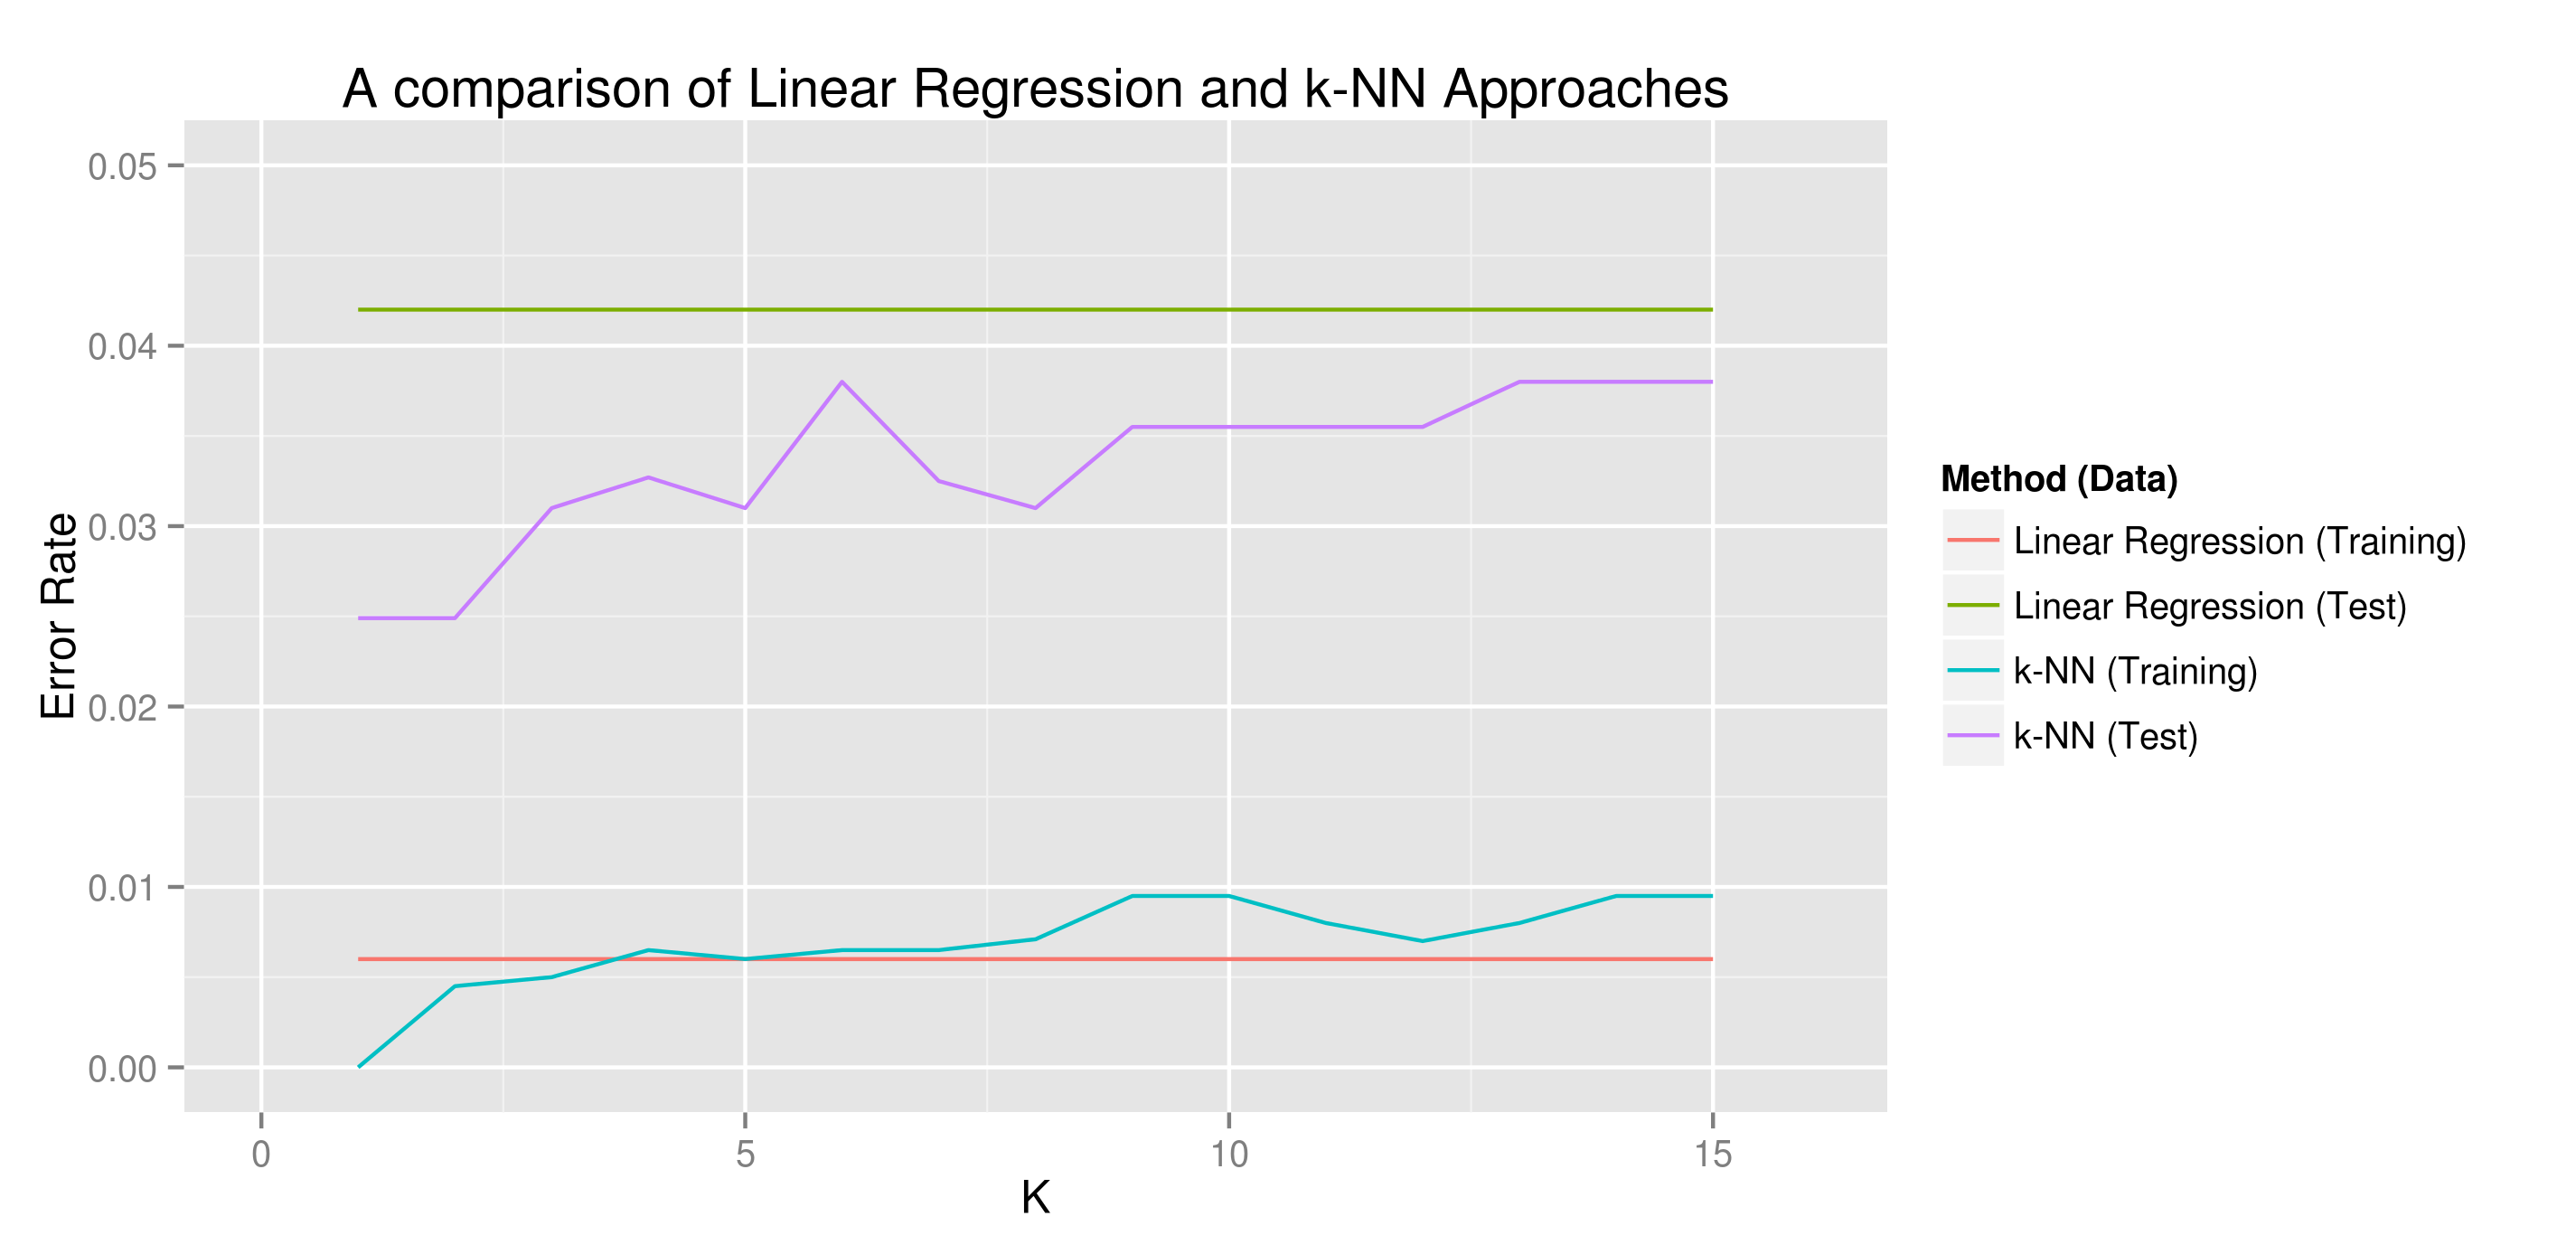
\includegraphics[width=.9\linewidth]{error_plot}
    \caption{A graphical comparison of the errors of the Linear Regression and the k-NN classification methods.}
    \label{fig:errors}
  \end{figure}

The R code used is as follows:
\begin{verbatim}
##
# ESL Exercise 2.8
#
##

######################
# some initial setup #
######################
working.directory = "~/Desktop/STAT775/HW01/Exercise_02_08"
training.file.name = "zip.test"
test.file.name = "zip.train"

setwd(working.directory)

require(ggplot2)
require(reshape)

####################
# Data Preparation #
####################
read.and.filter.data <- function(file.name) {
  #
  #
  # Args:
  #
  # Returns:
  #
  data = read.table(
    file.name,
    header = F,
    row.name = NULL
  )
  data = subset(data, V1 == 2 | V1 == 3)
  return(data)
}

separate.classes <- function(x) {
  if (x == 3) {
    return(1)
  } else {
    return(-1)
  }
}

zip.train <- read.and.filter.data(training.file.name)
training.data <- data.matrix(zip.train[, -1])
training.targets <- data.matrix(zip.train[, 1])
for (i in 1:length(training.targets)) {
  training.targets[i] <- separate.classes(training.targets[i])
}

zip.test <- read.and.filter.data(test.file.name)
test.data <- data.matrix(zip.train[, -1])
test.targets <- data.matrix(zip.train[, 1])
for (i in 1:length(test.targets)) {
  test.targets[i] <- separate.classes(test.targets[i])
}

k.range <- 1:15  # simpler than doing just 1, 3, 5, 7, 15
determine.category <- function(x) {
  if(x >= 0) {
    return(1)
  } else {
    return(-1)
  }
}

#####################
# Linear Regression #
#####################
least.squares <- function(x, y) {
  xt.x <- t(x) %*% x
  xt.x.inv <- solve(xt.x)
  full.mat <- xt.x.inv %*% t(x)
  regression.weights <- full.mat %*% y
  return(regression.weights)
}

linear.predict <- function(inputs, betas) {
  # sometimes the formula is listed as x^t * b, but our 'inputs' data already has each
  # test vector in a row when we pass it as a matrix (for this script)
  result <- inputs %*% betas
  result <- lapply(result, function(x) {return(determine.category(x))})
  return(result)
}

digit.model.weights <- least.squares(x = training.data, y = training.targets)

linear.training.predictions <- list()
for(i in 1:length(training.targets)) {
  linear.training.predictions[i] <- linear.predict(inputs = training.data[i, ], betas = digit.model.weights)
}
linear.test.predictions <- list()
for(i in 1:length(test.targets)) {
  linear.test.predictions[i] <- linear.predict(inputs = test.data[i, ], betas = digit.model.weights)
}


########
# K-NN #
########
euclidean.distance <- function(x, y) {
  diff <- x - y
  squares <- diff^2
  return(sqrt(sum(squares)))
}

my.knn.predict <- function(input.point, training.points, training.labels, k) {
  distances = NULL
  for (i in 1:length(training.points[, 1])) {
    distances[i] <- euclidean.distance(input.point, training.points[i, ])
  }
  
  category <- training.labels
  results <- data.frame(distances, category)
  results <- results[order(-distances), ]
  results <- results$category[1:k]
  
  return(determine.category(mean(results)))
}

knn.training.predictions <- matrix(0, length(k.range), length(training.targets))
knn.test.predictions <- matrix(0, length(k.range), length(test.targets))
for (k in k.range) {
  for (j in 1:length(training.targets)) {
    knn.training.predictions[k, j] <- my.knn.predict(
      input.point = training.data[j, ],
      training.points = training.data,
      training.labels = training.targets,
      k = k
    )
  }
}
for (k in k.range) {
  for (j in 1:length(test.targets)) {
    knn.test.predictions[k, j] <- my.knn.predict(
      input.point = test.data[j, ],
      training.points = training.data,
      training.labels = training.targets,
      k = k
    )
  }
}


######################
# Error Computations #
######################
compute.error.rate <- function(targets, predictions) {
  incorrect.predictions = 0
  for (i in 1:length(targets)) {
    if (targets[1] != predictions[i]) {
      incorrect.predictions <- (incorrect.predictions + 1)
    }
  }
  return(incorrect.predictions / length(targets))
}

linear.training.error.rates <- compute.error.rate(training.targets, linear.training.predictions)
linear.training.error.rates <- rep(linear.training.error.rates, 15)
linear.test.error.rates <- compute.error.rate(test.targets, linear.test.predictions)
linear.test.error.rates <- rep(linear.test.error.rates, 15)

knn.training.error.rates <- NULL
for (k in k.range) {
  knn.training.error.rates[k] <- compute.error.rate(training.targets, knn.training.predictions[k, ])
}
knn.test.error.rates <- NULL
for (k in k.range) {
  knn.test.error.rates[k] <- compute.error.rate(test.targets, knn.test.predictions[k, ])
}


errors.for.plotting <- data.frame(
  "K" = 1:15,
  "Linear (Training)" = linear.training.error.rates,
  "Linear (Test)" = linear.test.error.rates,
  "KNN (Training)" = knn.training.error.rates,
  "KNN (Test)" = knn.test.error.rates
)

############
# Plotting #
############

plot.data <- melt(errors.for.plotting, id = "K", variable_name = "Method")
ggplot(data = plot.data, aes(x = K, y = value, color = Method)) +
  geom_line() +
  ggtitle("A comparison of Linear Regression and k-NN Approaches") +
  xlab("K") +
  ylab("Error Rate") +
  ylim(0, 0.05) +
  xlim(0, 16) +
  scale_color_hue(
    name = "Method (Data)",
    labels = c(
      "Linear Regression (Training)",
      "Linear Regression (Test)",
      "k-NN (Training)",
      "k-NN (Test)"
    )
  )
ggsave('error_plot.png')
\end{verbatim}

\end{document}
